\section{Statechart diagrams} \label{sec:statechart}
Statechart diagrams are a useful way to get an overview over the lifetime of objects in the problem domain.
This section describes the state chart diagram of objects whose behaivour is both interesting and unique to the project.

\subsection{Approval Request}
The approval request is one of the most central concepts in the application.
When someone wants to create a new version of a document, they instantiate an approval request, which has a version object attached.
The change will have to be approved by all the users set as "approvers", before it can be added to the handbook.
When the change is approved, it will append the version to the document object.
For the sake of simplicity, there is no option to actually deny a proposed version.
Any issues with the document are, as mentioned in \cref{sec:richpictures}, meant to be handled outside of the system instead.
%mangler mulighed for delete

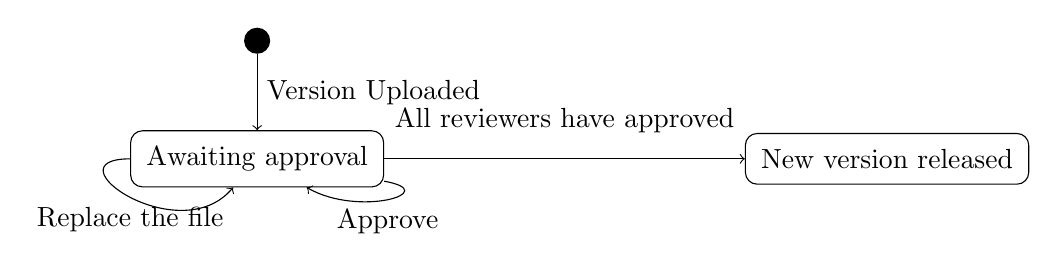
\begin{tikzpicture}[round/.style={rounded corners=1.5mm,minimum width=1cm,inner sep=2mm,above right,draw,align=left}]

	\node[circle, fill=black,minimum size=3pt] (start) {};
	\node[round] (await) [below of=start, node distance=1.5cm] {Awaiting approval};
	\path[->] (start) edge node[right] {Version Uploaded} (await);
	\path[->] (await) edge [loop below, out=350, in=330, looseness=2] node {Approve} (await);
	\path[->] (await) edge [loop below, out=180, in=230, looseness=2] node [distance=1cm] {Replace the file} (await);
	\node[round] (approved) [right of=await, node distance=8cm] {New version released};
	\path[->] (await) edge node[above, yshift=0.2cm] {All reviewers have approved} (approved);

\end{tikzpicture}

\subsection{Department}
A department is an organisational unit, used to administrate which users are attached to which documents.
As such, you can create a department, add users to it, and add documents to it.
It is also possible to delete users and documents from the department, as long as there are any attached to the department.
One of the most important functions of the department is the abillity for it to notify all the attached users of a new version of a document.
This was also the very reason the Department class was first made, see \cref{sec:Classes}
%tilføjet sætning ovenover -astrid

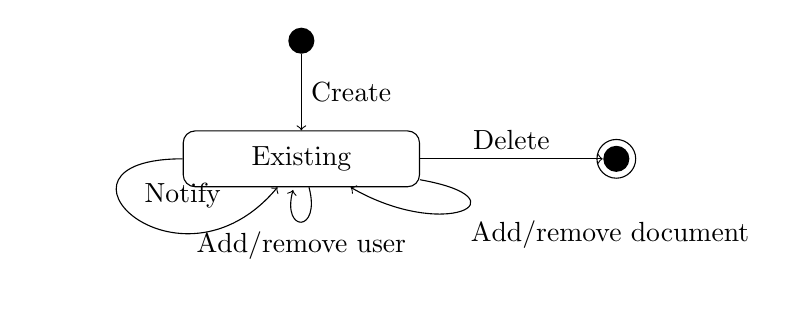
\begin{tikzpicture}[round/.style={rounded corners=1.5mm,minimum width=1cm,inner sep=2mm,above right,draw,align=left}]

	\node[circle, fill=black,minimum size=3pt] (start) {};
	\node[round, minimum width=3cm] (await) [below of=start, node distance=1.5cm] {Existing};
	\path[->] (start) edge node[right] {Create} (await);
	\path[->] (await) edge [loop below] node[auto] {Add/remove user} (await);
	\path[->] (await) edge [loop below, out=350, in=330, looseness=4] node[auto] {Add/remove document} (await);
	\path[->] (await) edge [loop below, out=180, in=230, looseness=4] node[auto] {Notify} (await);

	\draw[fill=white] circle[radius = 7pt, right of=await, node distance=4cm];
	\node[circle, fill=black,minimum size=3pt] (end) [right of=await, node distance=4cm] {};
	\path[->] (await) edge node[above] {Delete} (end);
%teksten Notify er ikke helt god -astrid

\end{tikzpicture}

\subsection{Version}
A version is another central concept in the application.
As mentioned before, the handbook consists of documents, and each document can have multiple versions.
And thus, after creation, version objects are supposed to be quite immutable once created, as to preserve the history of individual documents.
Due to the immutable structure of the versions, the actual versions never change.
On the contrary, by virtue of no longer being the last version in the document, they now count as archived.

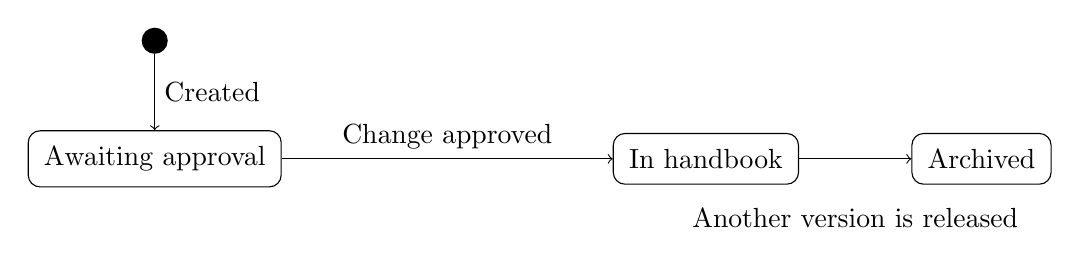
\begin{tikzpicture}[round/.style={rounded corners=1.5mm,minimum width=1cm,inner sep=2mm,above right,draw,align=left}]

	\node[circle, fill=black,minimum size=3pt] (start) {};
	\node[round] (await) [below of=start, node distance=1.5cm] {Awaiting approval};
	\path[->] (start) edge node[right] {Created} (await);
	\node[round] (approved) [right of=await, node distance=7cm] {In handbook};
	\path[->] (await) edge node[above] {Change approved} (approved);
	\node[round] (archived) [right of=approved, node distance=3.5cm] {Archived};
	\path[->] (approved) edge node[below, yshift=-0.5cm] {Another version is released} (archived);

\end{tikzpicture}
%re: Jan der siger at et objekts slutstadie er det stadie hvor det ikke længere kan paaføres eller udføre hændelser burde archived saa ikke være versions slutstadie???

\section{Scope of the problem domain}
% et eller andet om OOA&D er blevet brugt
The object oriented analysis principles were used throughout this chapter to analyze the different classes and events in the problem domain.
% et eller andet om qualified classes - ex. på qualified og ikke qualified classes
Classes like Document and Version were classified as qualified classes using the questions mentioned in \cref{sec:Classes} and classes like TOC and Notification were classified as not qualified classes.
% et eller andet om qualified events - ex. på qualified og ikke qualified event
Using the questions, mentioned in \cref{sec:Events}, Version approved and Department deleted were classified as qualified events whereas an event like Approval denied was classified as a not qualified event.
%lidt svært ved at forstaa pointen med det her afsnit??? -astrid (fuck hvor er jeg glad for at jeg ikke hedder aase)

% et eller andet om event table
An event table was made in \cref{sec:EventTable} using the classified classes and events, see \cref{fig:eventtable}.
This gave a better overview of what classes were affected by the different events.
% et eller andet om class diagram
The qualified classes specified in \cref{sec:Classes} were also used to produce a class diagram.
The class diagram describes the relation between the classes and objects, see \cref{fig:ClassDiagram} in \cref{sec:classdiagram}.
% et eller andet om state charts - ex. på nogle af de vigtigste events
Finally, the lifetime of some of the more important objects in the problem domain was described using state charts, see \cref{sec:statechart}.
The lifetime of e.g. the Department is that the department is being created and while it exists the department can:

\begin{itemize}
	\item Add and remove documents.
	\item Add and remove users.
	\item Notify users that a new version has been released.
\end{itemize}

The lifetime of the department ends when it is deleted.

% en meget hurtigt afrunding
The knowledge gained from analysing the problem domain makes it possible to examine how the actors interact with the system in the application domain in the next chapter.
